\documentclass[12pt]{article}
\usepackage[danish]{babel}
\usepackage{amsfonts, amssymb, mathtools, amsthm, amsmath}
\usepackage{graphicx, pgfplots}
\usepackage{url}
\usepackage[dvipsnames]{xcolor}
\usepackage{sagetex}
\usepackage{lastpage}

%loaded last
\usepackage[hidelinks]{hyperref}

\usepackage{siunitx}
  \sisetup{exponent-product = \cdot,
    output-decimal-marker = {,}}

%Giles Castelles incfig
\usepackage{import}
\usepackage{xifthen}
\usepackage{pdfpages}
\usepackage{transparent}

\newcommand{\incfig}[2][1]{%
  \def\svgwidth{#1\columnwidth}
  \import{../figures/}{#2.pdf_tex}
}

\setlength{\parindent}{0in}
\setlength{\oddsidemargin}{0in}
\setlength{\textwidth}{6.5in}
\setlength{\textheight}{8.8in}
\setlength{\topmargin}{0in}
\setlength{\headheight}{18pt}

\usepackage{fancyhdr}
\pagestyle{fancy}

\fancyhead{}
\fancyfoot{}
\fancyfoot[R]{\thepage}
\fancyhead[C]{\leftmark}

\pgfplotsset{compat=newest}

\pgfplotsset{every axis/.append style={
  axis x line=middle,    % put the x axis in the middle
  axis y line=middle,    % put the y axis in the middle
  axis line style={<->,color=black}, % arrows on the axis
}}

\usepackage{thmtools}
\usepackage{tcolorbox}
  \tcbuselibrary{skins, breakable}
  \tcbset{
    space to upper=1em,
    space to lower=1em,
  }

\theoremstyle{definition}

\newtcolorbox[auto counter]{definition}[1][]{%
  breakable,
  colframe=ForestGreen,  %frame color
  colback=ForestGreen!5, %background color
  colbacktitle=ForestGreen!25, %background color for title
  coltitle=ForestGreen!70!black,  %title color
  fonttitle=\bfseries\sffamily, %title font
  left=1em,              %space on left side in box,
  enhanced,              %more options
  frame hidden,          %hide frame
  borderline west={2pt}{0pt}{ForestGreen},  %display left line
  title=Definition \thetcbcounter: #1,
}

\newtcolorbox{greenline}{%
  breakable,
  colframe=ForestGreen,  %frame color
  colback=white,          %remove background color
  left=1em,              %space on left side in box
  enhanced,              %more options
  frame hidden,          %hide frame
  borderline west={2pt}{0pt}{ForestGreen},  %display left line
}

\newtcolorbox[auto counter, number within=section]{eks}[1][]{%
  brekable,
  colframe=NavyBlue,  %frame color
  colback=NavyBlue!5, %background color
  colbacktitle=NavyBlue!25,    %background color for title
  coltitle=NavyBlue!70!black,  %title color
  fonttitle=\bfseries\sffamily, %title font
  left=1em,            %space on left side in box,
  enhanced,            %more options
  frame hidden,        %hide frame
  borderline west={2pt}{0pt}{NavyBlue},  %display left line
  title=Eksempel \thetcbcounter: #1
}

\newtcolorbox{blueline}{%
  breakable,
  colframe=NavyBlue,     %frame color
  colback=white,         %remove background
  left=1em,              %space on left side in box,
  enhanced,              %more options
  frame hidden,          %hide frame
  borderline west={2pt}{0pt}{NavyBlue},  %display left line
}

\newtcolorbox{teo}[1][]{%
  breakable,
  colframe=RawSienna,  %frame color
  colback=RawSienna!5, %background color
  colbacktitle=RawSienna!25,    %background color for title
  coltitle=RawSienna!70!black,  %title color
  fonttitle=\bfseries\sffamily, %title font
  left=1em,              %space on left side in box,
  enhanced,              %more options
  frame hidden,          %hide frame
  borderline west={2pt}{0pt}{RawSienna},  %display left line
  title=Teori: #1,
}

\newtcolorbox[auto counter, number within=section]{sæt}[1][]{%
  breakable,
  colframe=RawSienna,  %frame color
  colback=RawSienna!5, %background color
  colbacktitle=RawSienna!25,    %background color for title
  coltitle=RawSienna!70!black,  %title color
  fonttitle=\bfseries\sffamily, %title font
  left=1em,              %space on left side in box,
  enhanced,              %more options
  frame hidden,          %hide frame
  borderline west={2pt}{0pt}{RawSienna},  %display left line
  title=Sætning \thetcbcounter: #1,
  before lower={\textbf{Bevis:}\par\vspace{0.5em}},
  colbacklower=RawSienna!25,
}

\newtcolorbox{redline}{%
  breakable,
  colframe=RawSienna,  %frame color
  colback=white,       %Remove background color
  left=1em,            %space on left side in box,
  enhanced,            %more options
  frame hidden,        %hide frame
  borderline west={2pt}{0pt}{RawSienna},  %display left line
}

\newtcolorbox{for}[1][]{%
  breakable,
  colframe=NavyBlue,  %frame color
  colback=NavyBlue!5, %background color
  colbacktitle=NavyBlue!25,    %background color for title
  coltitle=NavyBlue!70!black,  %title color
  fonttitle=\bfseries\sffamily, %title font
  left=1em,              %space on left side in box,
  enhanced,              %more options
  frame hidden,          %hide frame
  borderline west={2pt}{0pt}{NavyBlue},  %display left line
  title=Forklaring #1,
}

\newtcolorbox{bem}{%
  breakable,
  colframe=NavyBlue,  %frame color
  colback=NavyBlue!5, %background color
  colbacktitle=NavyBlue!25,    %background color for title
  coltitle=NavyBlue!70!black,  %title color
  fonttitle=\bfseries\sffamily, %title font
  left=1em,              %space on left side in box,
  enhanced,              %more options
  frame hidden,          %hide frame
  borderline west={2pt}{0pt}{NavyBlue},  %display left line
  title=Bemærkning:,
}

\makeatother
\def\@lecture{}%
\newcommand{\lecture}[3]{
  \ifthenelse{\isempty{#3}}{%
    \def\@lecture{Lecture #1}%
  }{%
    \def\@lecture{Lecture #1: #3}%
  }%
  \subsection*{\makebox[\textwidth][l]{\@lecture \hfill \normalfont\small\textsf{#2}}}
}

\makeatletter

\newcommand{\opgave}[1]{%
 \def\@opgave{#1}%
 \subsection*{Opgave #1}
}

\makeatother

%Format lim the same way in intext and in display
\let\svlim\lim\def\lim{\svlim\limits}

% horizontal rule
\newcommand\hr{
\noindent\rule[0.5ex]{\linewidth}{0.5pt}
}

\title{Afleveringsopgave til uge 25}
\author{Noah Rahbek Bigum Hansen}
\date{DATO}

\begin{document}

\maketitle

\section*{Opg. 14.5}
A machine part is undergoing SHM with a frequency of \qty{4,00}{Hz} and amplitude \qty{1,80}{cm}. How long does it take the part to go from $x = 0$ to $x = -\qty{1,80}{cm}$?
\bigbreak
Perioden for et objekt i SHM er den inverse frekvens. Vi får altså
\[ 
T = \frac{1}{f} = \frac{1}{\qty{4,00}{Hz}} = \qty{0,25}{s} 
.\]
Når maskindelen bevæger sig fra $x = 0$ til $x = a$ svarer det til at den har gennemløbet 1/4 periode. Altså er den samlede forbrugte tid
\[ 
t = \frac{T}{4} = \frac{\qty{0,25}{s}}{4} = \qty{0,0625}{s} 
.\]




\section*{Opg. 14.8}
In a physics lab, you attach a \qty{0,200}{kg} air-track glider to the end of an ideal spring of negligible mass and start it oscillating. The elapsed time from when the glider first moves through the equilibrium point to the second time it moves through that point is \qty{2,60}{s}. Find the spring’s force constant.
\bigbreak
Idet massen passerer igennem en halv periode på $t =\qty{2,60}{s}$ må den samlede periode være det dobbelte. Altså
\[ 
T = 2\cdot t = 2\cdot \qty{2,60}{s} = \qty{5,20}{s} 
.\]
Frekvensen er derfor
\[ 
  f = \frac{1}{T} = \frac{1}{\qty{5,20}{s}} = \qty{0,192}{Hz} 
.\]
Dette giver en vinkelfrekvens på
\[ 
\omega = 2\pi f = 2 \pi \cdot \qty{0,192}{Hz} = \qty{1,208}{\frac{rad}{s}} 
.\]
Vi har desuden at
\[ 
  k = \omega^2 \cdot m = \left( \qty{1,208}{\frac{rad}{s}}  \right)^2 \cdot \qty{0,200}{kg} = \qty{0,292}{\frac{N}{m}} 
.\]



\section*{Opg. 14.16}
A small block is attached to an ideal spring and is moving in SHM on a horizontal, frictionless surface. When the amplitude of the motion is \qty{0,090}{m}, it takes the block \qty{2,70}{s} to travel from $x = \qty{0,090}{m}$ to $x = - \qty{0,090}{m}$. If the amplitude is doubled, to \qty{0,180}{m}, how long does it take the block to travel

\subsection*{(a)}
From $x = \qty{0,180}{m}$ to $x = -\qty{0,180}{m}$ and
\bigbreak
I dette tilfælde vil perioden $T = 2 \cdot \qty{2,70}{s}$ være det samme som ovenfor idet periode er uafhængigt af amplitude. 


\subsection*{(b)}
from $x = \qty{0,090}{m}$ to $x = -\qty{0,090}{m}$
\bigbreak
Vi kan generelt finde positionen som
\[ 
x = A \cos \omega t
.\]
Vi sætter $x = A$ for $\omega t = 0$ og $x = -A$ for $\omega t = \pi$. Vi har da $\omega t = \frac{\pi}{3}$ for $x = \frac{1}{2}A$. Dette giver os
\[ 
\cos \left( \frac{\pi}{3} \right) = \frac{1}{2}, \qquad \text{og} \qquad \cos \left( \frac{2\pi}{3} \right) = -\frac{1}{2}
.\]
Dermed har vi at
\[ 
\omega \Delta t = \frac{\pi}{3} \implies \Delta t = \frac{\pi}{3\cdot \omega}
.\]
$\omega$ kan findes som
\[ 
\omega = \frac{2\pi}{T} = \frac{2\pi}{\qty{2,70}{s}} = \qty{1,16}{s^{-1}}
.\]
Vi får da at
\[ 
\Delta t = \frac{\pi}{3 \cdot \qty{1,16}{s^{-1}}} = \qty{0,9}{s} 
.\]



\section*{Opg. 14.28}
A harmonic oscillator has angular frequency $\omega$ and amplitude $A$.

\subsection*{(a)}
What are the magnitudes of the displacement and velocity when the elastic potential energy is equal to the kinetic energy? (Assume that $U = 0$ at equilibrium.)
\bigbreak
Vi har at
\[ 
K = U = \frac{1}{2}mv^2 = \frac{1}{2}kx^2
.\]
Vi har desuden den samlede energi som
\[ 
E = K + U = \frac{1}{2}kA^2
.\]
Dermed har vi for $K = U$ at
\[
  K = U = \frac{1}{2} E = \frac{1}{4} kA^2
.\]

Dermed får vi at
\begin{align*}
  \frac{1}{2}mv^2 &= \frac{1}{4}kA^2 \\
  v^2 &= \frac{1}{2} \frac{k}{m} A^2 \\
  v^2 &= \frac{1}{2} \omega^2 A^2 \\
  v &= \pm \frac{1}{\sqrt{2}} \omega A \\
  v &= \left| \frac{1}{\sqrt{2}}\omega A \right|
.\end{align*}
Dermed har vi fundet størrelsen på hastighedsvektoren. Det samme kan gøres med den potentielle energi for at finde størrelsen på positionsvektoren som
\begin{align*}
  U &= \frac{1}{4}kA^2 \\
  \frac{1}{2}kx^2 &= \frac{1}{4}kA^2 \\
  x^2 &= \frac{1}{2} A^2 \\
  x &= \pm \frac{1}{\sqrt{2}}A \\
  x &= \left| \frac{1}{\sqrt{2}}A \right|
.\end{align*}

\subsection*{(b)}
How often does this occur in each cycle? What is the time between occurrences?
\bigbreak
Vi har at $x = \frac{1}{\sqrt{2}}A$ netop to gange hver periode (på vejen fra $x = 0$ til $x = \frac{\pi}{2}$ og på vejen fra $x = \frac{\pi}{2}$ til $x = 0$.) Det samme gør sig gældende for $x = -\frac{1}{\sqrt{2}}A$ og dermed må det gælde at den kinetiske energi og den potentielle energi har samme størrelse netop 4 gange i hver periode. Vi kan generelt finde position som
\[ 
  x = A \cos \omega t
.\]
For at $A \cos \omega t = A \frac{1}{\sqrt{2}}$ må det gælde at $\cos \omega t = \frac{1}{\sqrt{2}}$. Vi har at $\cos \omega t = \frac{1}{\sqrt{2}}$ for $\omega t = \frac{\pi}{4}, \frac{3\pi}{4}, \frac{5\pi}{4}, \frac{7\pi}{4}$.
Vi får derfor, at 
\[ 
\omega \Delta t = \frac{\pi}{2}
.\]
Og dermed bliver tiden $\Delta t$
\[ 
  \Delta t = \frac{\pi}{2} \frac{1}{\omega}
.\]


\subsection*{(c)}
At an instant when the displacement is equal to $\frac{A}{2}$, what fraction of the total energy of the system is kinetic and what fraction is potential?
\bigbreak
Vi har at den samlede energi er
\[ 
E = \frac{1}{2}kA^2
.\]
Den potentielle energi er givet som
\[ 
U = \frac{1}{2}kx^2 \implies U = \frac{1}{2}k \frac{A^2}{4} = \frac{1}{4} \left( \frac{1}{2}kA^2 \right)
.\]
Dermed ses det hurtigt, at den potentielle energi udgør 1/4 af den samlede energi ved $x = \frac{A}{2}$ og dermed må den kinetiske energi udgøre 3/4 af den samlede energi.


\section*{Opg. 14.62}
An object is undergoing SHM with period \qty{0,300}{s} and amplitude \qty{6,00}{cm}. At $t = 0$ the object is instantaneously at rest at $x = \qty{6,00}{cm}$. Calculate the time it takes the object to go from $x = \qty{6,00}{cm}$ to $x = -\qty{1,50}{cm} $.
\bigbreak
Idet objektet er stillestående for $x = \qty{6,00e-2}{m}$ må det betyde at $A = \qty{6,00e-2}{m}$. Derudover er det oplyst at perioden er $T = \qty{0,300}{s}$. Vi kan finde vinkelhastigheden som
\[ 
\omega = \frac{2\pi}{T} = \frac{2\pi}{\qty{0,300}{s}} = \qty{20,94}{\frac{rad}{s}} 
.\]
Vi har at
\[ 
  \cos \omega t = \frac{x}{A} = \frac{\qty{-1,50}{cm}}{\qty{6,00}{cm}} = -\frac{1}{4}
.\]
Altså fås at
\begin{align*}
  \omega t &= \cos^{-1} -\frac{1}{4} \\
  t &= \frac{\cos^{-1} -\frac{1}{4}}{\omega} \\
  &= \frac{\cos^{-1} -\frac{1}{4}}{\qty{20,94}{s^{-1}}} \\
  &= \qty{0,087}{s}
.\end{align*}


\section*{Opg. 14.68}
\begin{figure} [ht]
  \centering
  \caption{}
  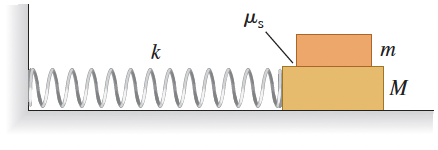
\includegraphics[width=0.5\linewidth]{../figures/F25_14_66.png}
  \label{fig:F25_14_66}
\end{figure}

Consider the system of two blocks and a spring shown in \textbf{\autoref{fig:F25_14_66}}. The horizontal surface is frictionless, but there is static friction between the two blocks. The spring has force constant $k = \qty{150}{\frac{N}{m}}$. The masses of the two blocks are $m = \qty{0,500}{kg}$ and $M = \qty{4,00}{kg}$. You set the blocks into motion by releasing block $M$ with the spring stretched a distance $d$ from equilibrium. You start with small values of $d$, and then repeat with successively larger values. For small values of $d$, the blocks move together in SHM. But for larger values of $d$, the top block slips relative to the bottom block when the bottom block is released.

\subsection*{(a)}
What is the period of the motion of the two blocks when $d$ is small enough to have no slipping?
\bigbreak
Først findes vinkelhastigheden som
\[ 
\omega = \sqrt{\frac{k}{m+M}} = \sqrt{\frac{\qty{150}{\frac{N}{m}}}{\qty{0,500}{kg} + \qty{4,00}{kg}}} = \qty{5,77}{s^{-1}} 
.\]
Dermed kan perioden findes som
\[ 
T = \frac{2\pi}{\omega} = \frac{2\pi}{\qty{33,33}{s^{-1}}} = \qty{1,09}{s} 
.\]


\subsection*{(b)}
The largest value $d$ can have and there be no slipping is $d = \qty{8,8}{cm}$. What is the coefficient of static friction $\mu_s$ between the surfaces of the two blocks?
\bigbreak
Vi har ved glidegrænsen at
\[ 
ma_{max} = m \mu g \implies a_{max} = \mu g
.\]
Vi har desuden accelerationen som
\[ 
a = \frac{k}{m}x \implies a_{max} = \frac{k}{m+M}x
.\]
Sættes udtrykkene for $a_{max}$ lig hinanden fås at
\begin{align*}
  \mu g &= \frac{k}{m+M}x \\
  \mu &= \frac{1}{g} \frac{k}{m+M}x \\
    &= \frac{1}{\qty{9,80}{\frac{m}{s^2}}} \cdot \frac{\qty{150}{\frac{N}{m}}}{\qty{4,50}{kg}} \cdot \qty{8,8e-2}{m} \\
    &= \num{0,299} \approx \num{0,3} 
.\end{align*}


\section*{Opg. 14.72}
\textbf{SHM of a Floating Object.} An object with height $h$, mass $M$, and a uniform cross-sectional area $A$ floats upright in a liquid with density $\rho$.

\subsection*{(a)}
Calculate the vertical distance from the surface of the liquid to the bottom of the floating object at equilibrium.
\bigbreak
Vi har hele volumenet af objektet som
\[ 
V = Ah
.\]
Hvis vi betegner den lodrette afstand fra overfladen af vandet til bunden af objektet $\ell$ fås det nedsunkne volumen som
\[
  V_{s} = A \ell
.\]
Idet der er statik må det gælde at
\[ 
F_g + F_b = 0
.\]
Altså har vi
\begin{align*}
  mg &= \rho g A \ell \\
  l &= \frac{m}{\rho A}
.\end{align*}



\subsection*{(b)}
A downward force with magnitude $F$ is applied to the top of the object. At the new equilibrium position, how much farther below the surface of the liquid is the bottom of the object than it was in part (a)? (Assume that some of the object remains above the surface of the liquid.)
\bigbreak
Idet vi sætter den ekstra afstand som objektet presses ned til $y$ har vi nu i stedet at
\begin{align*}
  mg + F &= \rho g A (\ell + y) \\
  \rho g A \ell + F &= \rho g A (\ell + y) \\
  F &= \rho g A y \\
  y &= \frac{F}{\rho g A}
.\end{align*}




\subsection*{(c)}
Your result in part (b) shows that if the force is suddenly removed, the object will oscillate up and down in SHM. Calculate the period of this motion in terms of the density $\rho$ of the liquid, the mass $M$, and the cross-sectional area $A$ of the object. You can ignore the damping due to fluid friction (see Section 14.7).
\bigbreak
Den effektive ``fjederkraft'' er
\[ 
F = \rho g A y
.\]
Af ovenstående kan ``fjederkonstanten'' aflæses til at være $k = \rho g A$ og altså kan vinkelhastigheden findes som
\[ 
\omega = \sqrt{\frac{k}{m}} = \sqrt{\frac{\rho g A}{m}}
.\]
Vi har desuden at 
\[ 
\omega = \frac{2\pi}{f}
.\]
Altså at
\begin{align*}
  2\pi f &= \sqrt{\frac{\rho g A}{m}} \\
  f &= \frac{1}{2\pi} \sqrt{\frac{\rho gA}{m}} \\
  T &= 2\pi \sqrt{\frac{m}{\rho gA}}
.\end{align*}


\end{document}
